%%%%% Description: consistency model history in terms of multiprocessor systems and distributed systems %%%%%
%%%%% Date: July 16, 2016 %%%%%
%%%%% Author: Hengfeng Wei (hengxin) %%%%%

\documentclass{standalone}

\usepackage{tikz}
\usetikzlibrary{positioning, shapes, shapes.symbols, backgrounds, fit, arrows.meta, calc}
\usepackage{varwidth}

\begin{document}
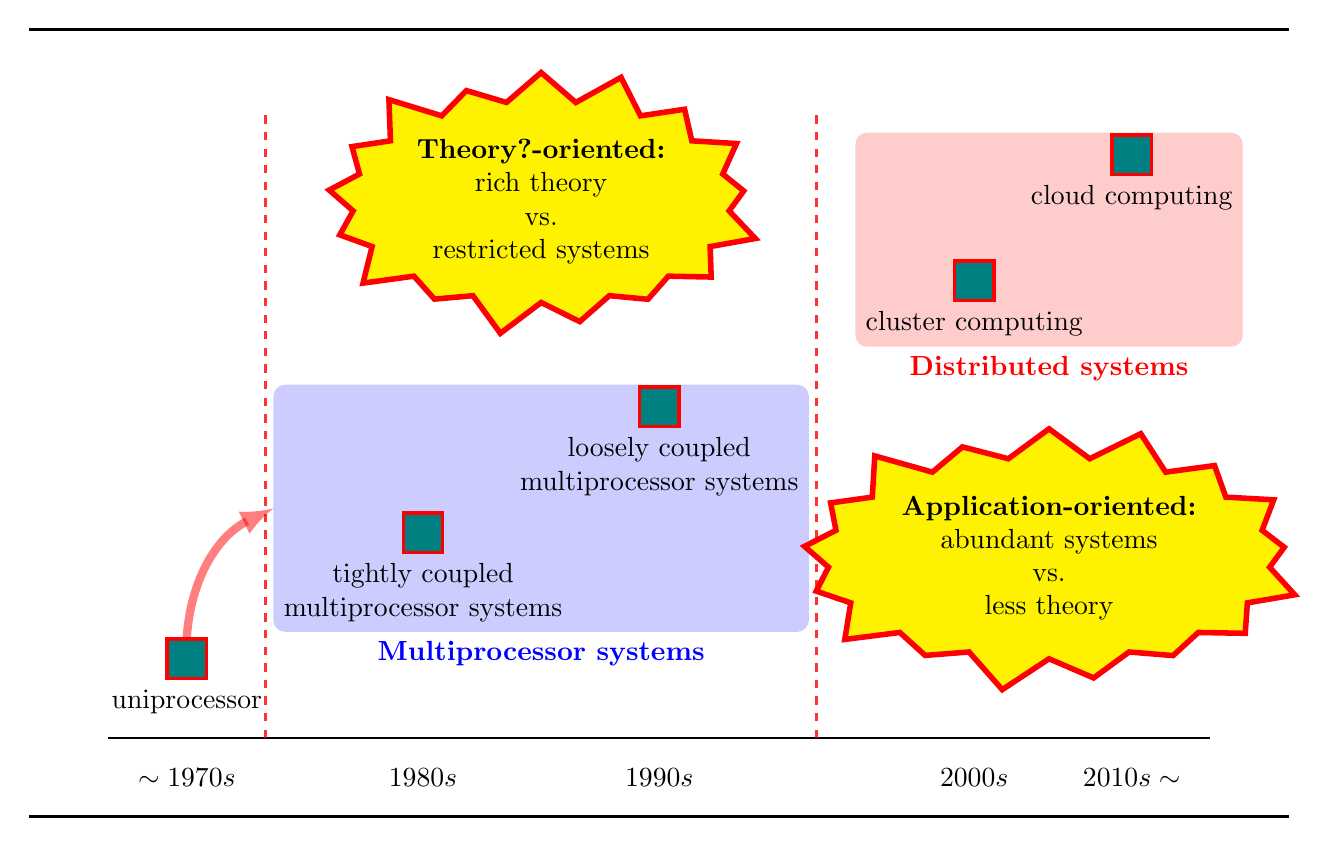
\begin{tikzpicture}[dnode/.style = {rectangle, minimum size = 0.50cm, fill = teal, draw = red, very thick},
	sepline/.style = {dashed, very thick, opacity = 0.80, red},
	comment/.style = {starburst, fill = yellow, draw = red, line width = 2pt, align = center}]

  %%%%%%%%%% begin %%%%%%%%%%  
  \draw[very thick] (0,0) to (16,0);  % the bottom line

  %%%%%%%%%% Begin: decades and systems %%%%%%%%%% 
  \draw[] (1,1) to (15,1);  % decade line

  % \y: y coordinate; \d: decade; \n: name; \slbl: system label; \sn: system name; \sln: system label name
  \foreach \y/\d/\n/\slbl/\sn/\sln [count = \yi] in {
  	2/$\sim 1970s$/70s/uniprocessor/uni/luni, 
	5/$1980s$/80s/tightly coupled \\ multiprocessor systems/tmul/ltmul, 
	8/$1990s$/90s/loosely coupled \\ multiprocessor systems/lmul/llmul, 
    12/$2000s$/00s/cluster computing/cluster/lcluster, 
    14/$2010s \sim$/10s/cloud computing/cloud/lcloud} {
    \node[] (\n) at (\y, 0.5) {\d};

	% \node[inner sep = 0pt, above = of \n] () {\includegraphics[width = 0.20\textwidth]{}};
	\node[dnode, above = (\yi-1) * 1.6 + 1 of \n, label = {[name = \sln, align = center] below : \slbl}] (\sn) {};  % try non-linear!!!
  }
  %%%%%%%%%% End: decades and systems %%%%%%%%%% 

  %%%%%%%%%% Begin: Multiprocessor systems %%%%%%%%%% 
  % multiprocessor system
  \begin{pgfonlayer}{background}
	\node[draw = blue!20, fill = blue!20, rectangle, rounded corners, inner sep = 0pt, fit = (tmul) (lmul) (ltmul) (llmul), 
	  label = {[blue] below : {\bf Multiprocessor systems}}] (mul) {};
  \end{pgfonlayer}

  % loosely coupled multiprocessor system
  % \node[above = 1.0cm of tmul] () {\includegraphics[scale = 0.40]{figs/tight-multiprocessor.png}};
  % \node[above = 2.0cm of lmul] () {\includegraphics[scale = 0.40]{figs/loose-multiprocessor.png}};

  % from uniprocessor system to multiprocessor system
  \draw[sepline] (3.0, 1.0) to (3.0, 9.0);
  \draw[-latex, line width = 3pt, red, opacity = 0.5] (uni.north) to [bend left] (mul.west);
  %%%%%%%%%% End: Multiprocessor systems %%%%%%%%%% 

  %%%%%%%%%% Begin: Consistency models %%%%%%%%%% 
  % lots of consistency models (TODO: another frame page and another tikz file)

  % comment on consistency models in the context of multiprocessor systems
  \node[above = of mul, comment] (multi-comment) {{\bf Theory?-oriented:}\\ rich theory \\ vs. \\ restricted systems};

  % separation line: from multiprocessor to WAN apps
  \draw[sepline] (10.0, 1.0) to (10.0, 9.0);
  %%%%%%%%%% End: Consistency models %%%%%%%%%% 

  % multiprocessor system
  \begin{pgfonlayer}{background}
	\node[draw = red!20, fill = red!20, rectangle, rounded corners, inner sep = 0pt, fit = (cluster) (lcluster) (cloud) (lcloud), 
	  label = {[red] below : {\bf Distributed systems}}] (dissys) {};
  \end{pgfonlayer}

  % comment on consistency models in the context of ???
  \node[below = of dissys, comment] (comment-multi) {{\bf Application-oriented:}\\ abundant systems \\ vs. \\ less theory};
  \draw[very thick] (0,10) to (16,10);  % the top line
\end{tikzpicture}

\end{document}